\chapter{Motivation}\label{chp:motivation}
% Authors: Ethan Perez, Diego Casabuena, Yi Tang. 2/3/18.

\section{Ideas for “Generic” Feature Extraction}\label{ssec:generic-feature-extraction}
% Authors: Ethan Perez, Diego Casabuena, Yi Tang. 2/3/18.

For much of its history, the field of Artificial Intelligence has viewed high-quality hand-crafted, task-specific features as the key to machine intelligence.
In contrast, more recent years have witnessed the popularity and successes of \textit{learned} and generic features.
Preceding deep learning, many other approaches (such as SVM) for extracting generic features have been explored.

Generally speaking, feature extraction often consists of expanding the input's representational dimension such that the expanded features are more likely to be linearly separable; intuitively, points in higher dimensional space are more likely to be linearly separable due to the increase in the number of possible separating planes.
To this end, feature extracting algorithms may learn some $f(x)=\sum_i w_i \phi_i (x)$, where $w_i$ are the learned coefficients and $\phi_i$ are some chosen basic features.
To form $\phi_i (x)$, there are (among others) five common approaches:

\begin{enumerate}
    \item \textbf{Space tiling}: To use linear combinations of engineered features.
    In this method $\phi_i(x) = \phi(x,u_i)$ are used where $u_i$ spreads over the domain.
    However, this method does not scale that well in the number of input dimensions $d$, as one would need $n^d$ bumps/mappings/sub-functions to spread a grid of size $n$ in each dimension.

    \item \textbf{Random projections}: To compose random projection matrices and use them to get features.
    Randomly projected features turn out to perform well in practice.

    \item \textbf{Polynomial classifier}: To use monomials as $\phi_i$.
    This is a very common method of involving additional dimensions.
    Given data of dimension $d$, one can compose a polynomial whose terms are the products of particular dimensions.
    For example, for $d = 2$ (and data $(x_1, x_2)$), the polynomial would assume the form
    \begin{equation*}
        w_0 + \sum_{a \in \mathbb{N}^*} w_{1, a} x_1^a + \sum_{b \in \mathbb{N}^*} w_{2, b} x_2^b + \sum_{c_1, c_2 \in \mathbb{N}^*} w_{3, c_1, c_2} x_1^{c_1} x_2^{c_2}
        \text{.}
    \end{equation*}
    % Doesn’t scale well in high dimensions.
    % Need to compute polynomial features of your input (how many are there?)
    One can further limit the degree of the polynomial for computational efficiency.
    For instance, a degree-2 polynomial (for $d = 2$) would have the form $w_0 + w_{1, 1} x_1 + w_{2, 1} x_2 + w_{1, 2} x_1^2 + w_{2, 2} x_2^2 + w_3 x_1 x_2$.

    \item \textbf{Radial Basis Functions (RBF)}: To use functions whose value depends only on the distance from the variable to a given point.
    For example, a commonly used function family is $\phi_i(x)=e^{-{\|x-u_i\|}^2}$.

    \item \textbf{Kernel machines}: Based on a kernel function that satisfies the Mercer condition.
    More specifically, one could use $\phi_i(x) = K(x, u_i)$ where $K$ is a continuous, symmetric, positive-definite kernel function (which indicates the matrix $[K(x_i, x_j)]_{i, j}$ is positive definite, where $x_i$ are the sample points).
    In essence, taking $\phi_i(x) = K(x, x_i)$ is equivalent to a 2-layer neural network that uses tiling, that locates exactly around the training sample points (as $u_i = x_i$).
\end{enumerate}

As a sidenote, it is not hard to see how a single layer classifier of the sorts discussed above may potentially require infinite dimensions.

\section{History of Deep Learning}\label{ssec:history}
% Authors: Ethan Perez, Diego Casabuena, Yi Tang. 2/3/18.

The seeds of deep learning date back at least to the invention of the perceptron by Frank Rosenblatt in 1957.
The perceptron is a binary classifier that attempts to linearly separate the data via weights on the input features learned via supervision.
The perceptron may be viewed as a single-layer neural network, and initially it seemed to be a promising statistical learning approach for classification problems (e.g., image classification).
However, in 1969, Marvin Minksy and Seymour Papert showed that perceptrons cannot compute or represent some functions, for example the XOR function.
This result only held for single-layer, linear perceptrons, and not in the case of non-linear multi-layer perceptrons.
Despite the potential of the perceptron, the above result discouraged further research into the method.
Thus, the field as it was known died and its place in research was taken by the related (or rebranded) fields of statistical learning theory and adaptive filters.
These would continue to make further developments in the following years.

In the early 1980s, several exciting results re-popularized neural networks for some time.
In 1982, John Hopfield discovered interesting mathematical connections between perceptrons (more generally neural networks) and concepts in physics.
Soon after, in 1983, Geoffrey Hinton developed the Boltzmann machine, publishing the method in AAAI, a top tier conference in AI at the time, in a paper titled ``\href{https://papers.cnl.salk.edu/PDFs/Optimal\%20Perceptual\%20Inference\%201983-646.pdf}{Optimal Perceptual Inference}.''
% Paper URL: https://papers.cnl.salk.edu/PDFs/Optimal%20Perceptual%20Inference%201983-646.pdf
The Boltzmann machine was one of the first methods that could train a \textit{multi-layer} perceptron.
Later, in 1985, Rumelhart, Hinton, Lecun, and several others discovered the backpropagation algorithm for training multi-layer perceptrons.
Backpropagation is conceptually simple: repeatedly apply the chain rule starting from the gradients of the last layer of the perceptron until the first layer.
Interestingly, this algorithm had not been discovered before this time, given that previous neural networks had largely been formulated with binary, thresholding activations, which are non-differentiable.
However, these activations could be swapped for other differentiable activations, such as sigmoid functions (a kind of soft thresholding function) or rectified linear units, in order to facilitate backpropagation.
Notably, this non-linear optimization procedure faces the theoretical problem of reaching local minima.
However, Hinton showed it was possible to successfully train neural nets anyways -- that in practice, the solutions found by backpropagation perform reasonably well.

Despite these successes, other models (such as the Support Vector Machine) in the 1990s and 2000s overtook neural networks in popularity.
It was not until the early 2010s that deep learning became popular yet again, with breakthrough successes in speech recognition and image classification.

\section{Hierarchical Representation}\label{ssec:hierarchical-representation}
% Authors: Ethan Perez, Diego Casabuena, Yi Tang. 2/3/18.

Deep learning has a hierarchical nature.
From simpler structures we derive more complex ones.
In a neural network, the layers are essentially stages of non-linear feature transformations.
This inherent hierarchy of representations can also be found on the Mammalian Visual Cortex, where the different sections of the Cortex understand increasingly complex levels of information about a visual input (as can be seen in \cref{fig:deep-learning-hierarchical-features}).

\begin{figure}[ht]
\centering
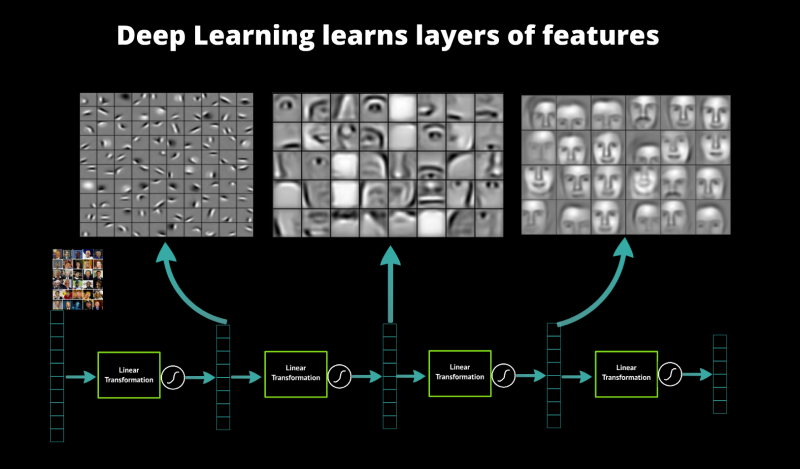
\includegraphics[width=0.85\linewidth]{lectures/01-a/dl_features.png}
% Figure from: https://www.datasciencecentral.com/profiles/blogs/a-primer-on-deep-learning
\caption{In the figure above we see how the layers closer to the input of the network are more abstract, and that those closer to the final layer are most concrete and interpretable.}
\label{fig:deep-learning-hierarchical-features}
\end{figure}

In a neural network, we feed the output of one layer onto the input of the next.
Layers are composed of linear transformations followed by non-linear activation functions.
Altogether, this system allows the network to learn the non-linear features of interest.

Hierarchical feature representations are intuitive for many domains, as our world is compositional (the whole is often a function of its parts).
For example, consider the following domains:
\begin{itemize}
    \item \textbf{Image recognition}: Pixels compose edges, which compose ``textons'' (i.e., multi-edge shapes), which compose motifs, which compose parts, which finally compose whole objects.
    Algorithms may learn to understand what an object looks like by learning a function mapping from pixels to a slightly higher level representation such as edges, then to textons, etc., until a high enough level representation is formed to represent whole objects.
    Indeed, there is evidence from neuroscience that the visual cortex represents objects in such a hierarchical manner in animals.

    \item \textbf{Language}: Language is inherently compositional as well.
    The meaning of a book is a composition of the meanings of its chapters, then paragraphs, then sentences, then phrases, then words (then even characters).
    While not all language is compositional (a ``heavy accent'' has nothing to do with weight), it often is, as language is how humans represent the world which is often compositional.

    \item \textbf{Speech}: In speech, a sample composes a band, which composes a sound, which compose phones, then phonemes, then whole words and sentences.
    The capacity for each component of this hierarchy in speech is what enables hierarchical models to represent very high-level features of sound by simply forming consecutively higher representations over what is ultimately a series of bytes.
\end{itemize}
